\documentclass[hyperref={pdfpagelabels=false}]{beamer}

\usepackage{listings}
\usepackage{algorithm}
\usepackage{ulem}
\usepackage{algorithmicx}
\usepackage{algpseudocode}

\definecolor{red}{rgb}{1,0,0}

\normalem

\usetheme{Warsaw}
\setbeamercovered{transparent}
\setbeamertemplate{footline}[page number]
\setbeamertemplate{navigation symbols}{} %remove navigation symbols
\setbeamertemplate{bibliography entry title}{}

\newcommand{\codestyle}{\small\sffamily}

% "define" Scala
\lstdefinelanguage{scala}{
  alsoletter={@,=,>},
  morekeywords={abstract, case, catch, class, def, do, else, extends, false, final, finally, for, if, implicit, import, match, new, null, object, 
override, package, private, protected, requires, return, sealed, super, this, throw, trait, try, true, type, val, var, while, with, yield, domain, 
postcondition, precondition,invariant, constraint, assert, forAll, in, _, return, @generator, ensure, require, holds, ensuring,=>},
  sensitive=true,
  morecomment=[l]{//},
  morecomment=[s]{/*}{*/},
  morestring=[b]"
}
\lstset{
%  frame=tb,
  language=scala,
%  aboveskip=3mm,
%  belowskip=3mm,
%  lineskip=-0.1em,
  escapeinside={\%}{\%},
  showstringspaces=false,
  columns=fullflexible,
  mathescape=true,
  numbers=none,
  numberstyle=\tiny,
  basicstyle=\codestyle
} 

\newcommand\highlight[1]{\color{red}{#1}}

\begin{document}
\title{Insane: Precise and Compositional Effect Analysis of Higher-Order Programs}
\author{Etienne Kneuss}
\date{\today}

\nocite{*}

\institute[EPFL]{
Laboratory for Automated Reasoning and Analysis \\
School of Computer and Communication Sciences\\
EPFL\\
}

\begin{frame}
    \titlepage
\end{frame}

%\section*{Outline}
%\begin{frame}
%    \frametitle{Outline}
%    \tableofcontents
%\end{frame}

\section{Introduction}

\begin{frame}[label=overview]
    \begin{figure}[t]
        
\includegraphics[width=60mm]{../../../logo.png}\\
        Interprocedural Static Analysis Engine for Scala
    \end{figure}

    \begin{itemize}
        \item Precise pointer and effect analysis
            \begin{itemize}
                \item Interprocedural
                \item Flow sensitive
                \item No annotations required
                \item Compositional
                \item Flexible representation of effects
                \item Designed for higher-order functions
            \end{itemize}
    \end{itemize}
\end{frame}

\begin{frame}
\frametitle{End Goal}
    Statically compute compositional summaries of
    \begin{enumerate}
        \item memory effects
        \item aliasing relations
    \end{enumerate}

    \vspace{25pt}
    For each method, we want to compute a summary that, given an abstract heap
    before the call, will allow the computation of a sound yet precise abstract
    heap after the call.
\end{frame}

\begin{frame}
\frametitle{Abstract Heaps}
  \begin{columns}
    \begin{column}{0.4\textwidth}

        Abstract Heaps: $H$
        \begin{itemize}
            \item Nodes are objects
            \item Edges are fields
        \end{itemize}

        \vspace{10pt}
        Method Summary:
        $S : (H, Par) \rightarrow (H, Ret)$


    \end{column}
    \begin{column}{0.6\textwidth}
      \begin{figure}[t]
            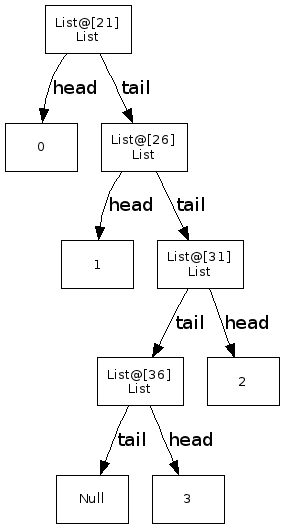
\includegraphics[height=60mm]{images/heap.png}\\
      \end{figure}
    \end{column}
  \end{columns}
\end{frame}

\begin{frame}
\frametitle{Simple Method Summaries: Requirements}
  Summaries are represented as graphs.

  \vspace{15pt}
  They express how the heap changed, and may refer to values that were
  only reachable before the method call.

  \vspace{15pt}
  They refer to objects that are unknown at the moment: parameters, \emph{this}.

\end{frame}
\subsection{Representation}

\begin{frame}[fragile]
\frametitle{Simple Example}
  \begin{columns}
    \begin{column}{0.4\textwidth}
\begin{lstlisting}
object Test {
  def run(l1: List,
          l2: List): List = {
    val old = l1.tail
    l1.tail = l2
    old
    %\color{red}{$\bigodot$}%
  }

  def test() = {
    val l = new List(0,
              new List(1,
               null))
    run(l, l)
    l
  }
}
\end{lstlisting}
    \end{column}
    \begin{column}{0.6\textwidth}
      \begin{figure}[t]
        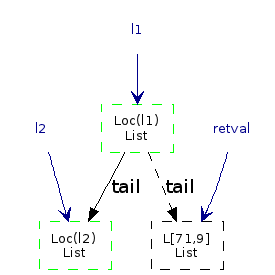
\includegraphics[width=40mm]{images/run_sum.png}\\
      \end{figure}
    \end{column}
  \end{columns}
\end{frame}

\begin{frame}[fragile]
\frametitle{Simple Example}
  \begin{columns}
    \begin{column}{0.4\textwidth}
\begin{lstlisting}
object Test {
  def run(l1: List,
          l2: List): List = {
    val old = l1.tail
    l1.tail = l2
    old
  }

  def test() = {
    val l = new List(0,
              new List(1,
               null))
    %\color{red}{$\bigodot$}%
    run(l, l)
    l
  }
}
\end{lstlisting}
    \end{column}
    \begin{column}{0.6\textwidth}
      \begin{figure}[t]
        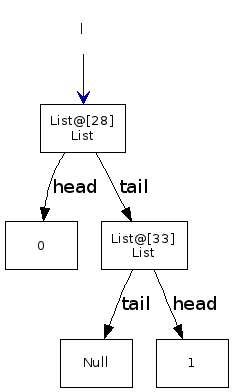
\includegraphics[height=50mm]{images/bef.png}\\
      \end{figure}
    \end{column}
  \end{columns}
\end{frame}

\begin{frame}[fragile]
\frametitle{Simple Example}
  \begin{columns}
    \begin{column}{0.3\textwidth}
      \begin{figure}[t]
        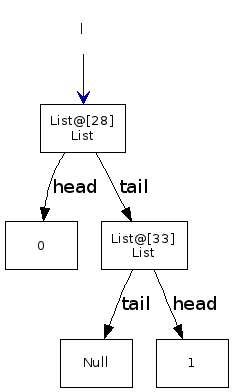
\includegraphics[height=40mm]{images/bef.png}\\
        \vspace{15pt}
        Before run()
      \end{figure}
    \end{column}
    \begin{column}{0.4\textwidth}
      \begin{figure}[t]
        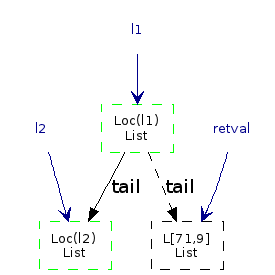
\includegraphics[height=30mm]{images/run_sum.png}\\
        \vspace{15pt}
        Method Summary
      \end{figure}
    \end{column}
    \begin{column}{0.3\textwidth}
      \begin{figure}[t]
        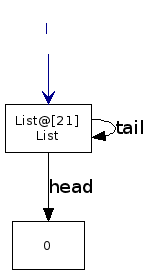
\includegraphics[height=35mm]{images/aft.png}\\
        \vspace{15pt}
        Result
      \end{figure}
    \end{column}
  \end{columns}
\end{frame}

\begin{frame}[fragile]
\frametitle{Method Summaries}
    The method summaries remain \textbf{abstractions}:
    \begin{itemize}
        \item not path sensitive
        \item order of writes/reads is lost
        \item we enforce a maximum depth for load nodes
        \item fresh objects are identified by their allocation site

    \end{itemize}
%  \begin{columns}
%    \begin{column}{0.4\textwidth}
%\begin{lstlisting}[escapechar=\%]
%  def f(l: List) = {
%    var c = l
%    while(c.next != null) {
%      c = c.next
%    }
%    c
%  }
%\end{lstlisting}
%    \end{column}
%    \begin{column}{0.6\textwidth}
%      \begin{figure}[t]
%        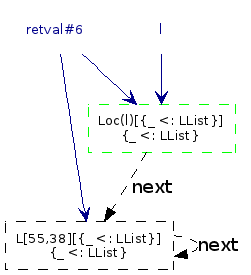
\includegraphics[height=30mm]{images/e6.png}\\
%      \end{figure}
%    \end{column}
%  \end{columns}
\end{frame}

\subsection{Problem?}
\begin{frame}[fragile]
\frametitle{First Challenge}
\begin{lstlisting}[escapechar=\%]
class List(var head: Int,
           var tail: List) {
  def mapHead(f: %\highlight{Int $\Rightarrow$ Int}%) = {
    List(%\highlight{f(head)}%, tail)
  }
}
\end{lstlisting}

    \vspace{10pt}
    How can we summarize \emph{mapHead()}?
\end{frame}

%\begin{frame}[fragile]
%\frametitle{First Challenge}
%\begin{lstlisting}[escapechar=\%]
%class List(var data: Int,
%           var next: List) {
%  def mapHead(f: %\highlight{F1[Int, Int]}%) = {
%    List(%\highlight{f.apply(data)}%, next)
%  }
%}
%\end{lstlisting}
%
%    \vspace{10pt}
%    How can we summarize \emph{mapHead()}?
%\end{frame}

\begin{frame}[fragile]
\frametitle{First Challenge}
    Two alternatives: 
    \vspace{15pt}

    \textbf{1: Considering all defined targets:}\\
    \vspace{5pt}
    Impossible in most cases: it kills precision.
    ($>$1K targets in the library)

    \vspace{15pt}
    \pause

    \textbf{2: Delay the analysis of \emph{f.apply}:}\\
    \vspace{5pt}
    Instead of analysing the call, we record in the summary that \emph{f.apply}
    was called.

\end{frame}


\section{New Representation}
\subsection{One Solution}
\begin{frame}[fragile]
\frametitle{New Effect Representation}
    Instead of generating simple effect graphs we:
    \begin{enumerate}
        \item Start from the CFG
        \item Analyze the precise parts of it
        \item Reduce the CFG by introducing \emph{effect statements} summarizing
        blocks of analyzed statements
    \end{enumerate}

    \vspace{15pt}
    \pause

    We obtain a CFG where only imprecise method calls remain! We use this
    reduced CFG as summary.

\end{frame}

\begin{frame}[fragile]
\frametitle{New Effect Representation: Flexibility}
    This representation is very flexible.

    We have at our disposal a very wide spectrum of precision.

    \vspace{15pt}

    \begin{figure}[t]
      \begin{center}
      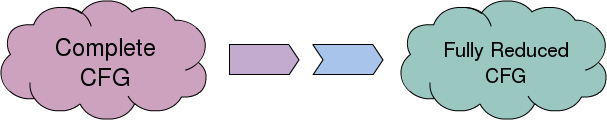
\includegraphics[width=60mm]{images/spectrum.png}\\
      \end{center}
    \end{figure}
\end{frame}

\begin{frame}[fragile]
\frametitle{New Effect Representation: Heuristics}
    How can we automatically decide when to leave the call unanalyzed?

    \vspace{15pt}
    $\Rightarrow$ We rely on score based heuristics.

    \vspace{15pt}
    Multiple ideas on how to compute the score:
    \begin{itemize}
        \item How many targets?
        \item Is the receiver reachable from method arguments?
        \item Can the precision of the receiver improve?
    \end{itemize}
\end{frame}

\subsection{Recap}
\begin{frame}[label=overview]
    \begin{figure}[t]
        
\includegraphics[width=60mm]{../../../logo.png}\\
        Interprocedural Static Analysis Engine for Scala
    \end{figure}

    \begin{itemize}
        \item Precise pointer and effect analysis
            \begin{itemize}
                \item Interprocedural
                \item Flow sensitive
                \item No annotations required
                \item Compositional
                \item Flexible representation of effects
                \item Designed for higher-order functions
            \end{itemize}
    \end{itemize}
\end{frame}
\begin{frame}[fragile]
    \begin{figure}
    \begin{center}
    Thanks
    \end{center}
    \end{figure}
\end{frame}
\appendix
\newcounter{finalframe}
\setcounter{finalframe}{\value{framenumber}}

%
%
% BACKUP SLIDES
%
%


\begin{frame}[fragile]
\frametitle{New Effect Representation: Difficulties}
    There is few difficulties when dealing with CFGs as summaries:
    \begin{itemize}
        \item The CFG under analysis gets modified when inlining the CFG
        corresponding to a method call.\\
            $\Rightarrow$ we discard some of the analysis state and partially restart with the new CFG

        \item The targets of method calls in loops can increase over iterations.\\
            $\Rightarrow$ we cannot simply replace the method call statement with the target CFG

        \item Monotonicity is not ensured in general.\\
            $\Rightarrow$ we have to ensure it by taking specific care of
            recursive methods.
    \end{itemize}
\end{frame}

\begin{frame}[fragile]
\frametitle{First Challenge: Delaying}
\begin{lstlisting}[escapechar=\%]
class C(var field1: C, var field2: C);
\end{lstlisting}

\begin{lstlisting}[escapechar=\%]
def plop1(obj: C, f: C $\Rightarrow$ Unit) = {
    obj.field1 = ..
    %\highlight{f(obj)}%
}

def plop2(obj: C, f: C $\Rightarrow$ Unit) = {
    %\highlight{f(obj)}%
    obj.field1 = ..
}
\end{lstlisting}
    \begin{figure}
    \center{
    $S(plop1) =^? S(plop2)$
\pause
\\
\textbf{no}, we want flow-sensitivity
\pause
    \\
    $\Rightarrow$ we need a new representation
    }
    \end{figure}
\end{frame}
\begin{frame}[fragile]
\frametitle{Example}
  \begin{columns}
    \begin{column}{0.4\textwidth}
\begin{lstlisting}[escapechar=\%]
class List(var data: Int,
           var next: List) {
  def mapHead(f: F1[Int, Int]) = {
    new List(f.apply(data), next)
  }
}
\end{lstlisting}
    \end{column}
    \begin{column}{0.6\textwidth}
      \begin{figure}[t]
%        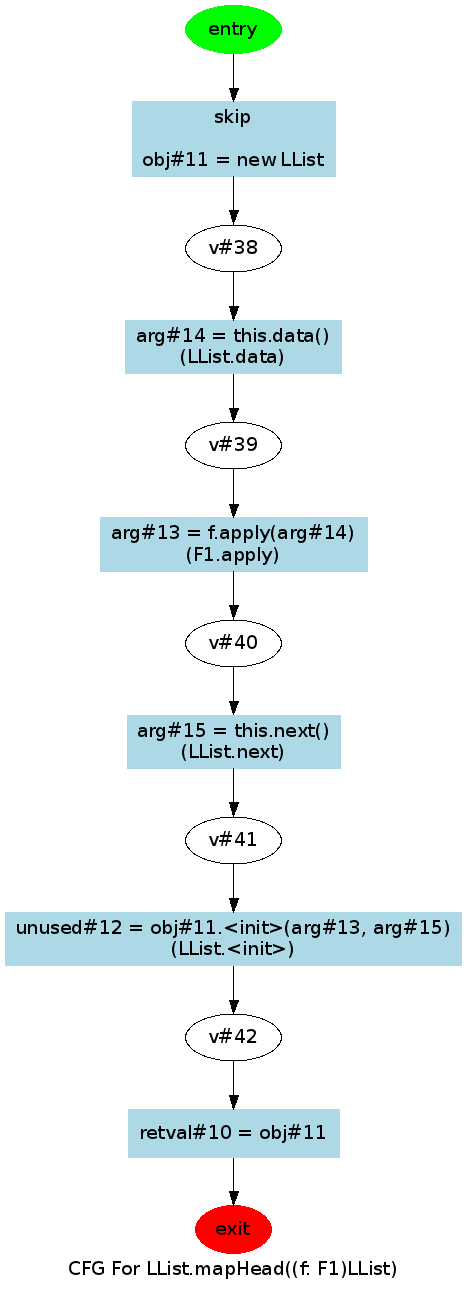
\includegraphics[height=60mm]{images/e3.png}\\
      \end{figure}
    \end{column}
  \end{columns}
\end{frame}
\begin{frame}[fragile]
\frametitle{Example}
  \begin{columns}
    \begin{column}{0.4\textwidth}
\begin{lstlisting}[escapechar=\%]
class List(var data: Int,
           var next: List) {
  def mapHead(f: F1[Int, Int]) = {
    val ll = new List
    ll.<init>(f.apply(this.data()), this.next())
    ll
  }
}
\end{lstlisting}
    \end{column}
    \begin{column}{0.6\textwidth}
      \begin{figure}[t]
        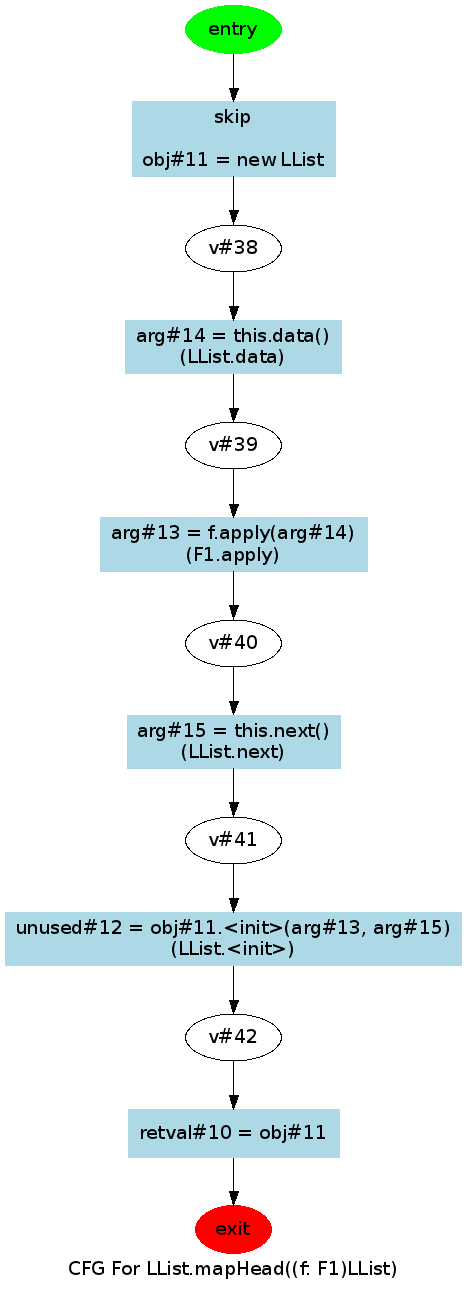
\includegraphics[height=60mm]{images/e3.png}\\
      \end{figure}
    \end{column}
  \end{columns}
\end{frame}

\begin{frame}[fragile]
\frametitle{Example}
  \begin{figure}[t]
    \begin{center}
    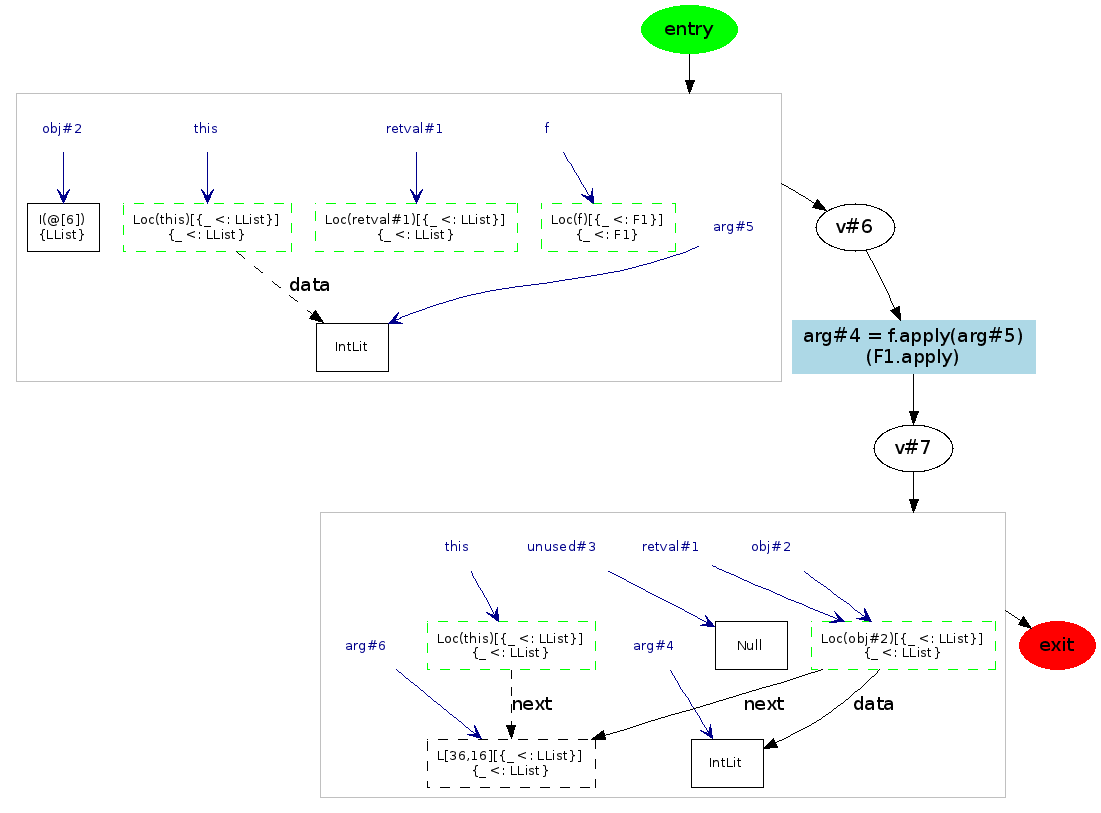
\includegraphics[width=90mm]{images/e4.png}\\
    \end{center}
  \end{figure}
\end{frame}

\begin{frame}[fragile]
\frametitle{Example}
  \begin{columns}
    \begin{column}{0.4\textwidth}
\begin{lstlisting}[escapechar=\%]
class List(var data: Int,
           var next: List) {
  def mapHead(f: F1[Int, Int]) = {
    val ll = new List
    ll.<init>(f.apply(this.data()), this.next())
    ll
  }
}

object Test {
  def test(l: List) = {
    l.mapHead({ i $\Rightarrow$ 42 })
  }
}
\end{lstlisting}
    \end{column}
    \begin{column}{0.6\textwidth}
      \begin{figure}[t]
        \begin{center}
        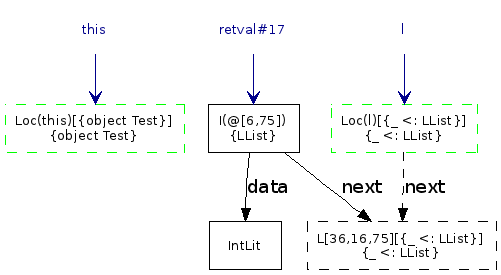
\includegraphics[width=60mm]{images/e5.png}\\
        Test.test()
        \end{center}
      \end{figure}
    \end{column}
  \end{columns}
\end{frame}





\end{document}
